\icode{N24X-MD-SI-L2-261111-001}
\nceeID[4]{2024湖南}{3}
如图，质量分别为\(4m\)、\(3m\)、\(2m\)、\(m\)的四个小球\(A\)、\(B\)、\(C\)、\(D\)，通过细线或轻弹簧互相连接，悬挂于\(O\)点，处于静止状态，重力加速度为\(g\)。若将\(B\)、\(C\)间的细线剪断，则剪断瞬间\(B\)和\(C\)的加速度大小分别为\paren[]

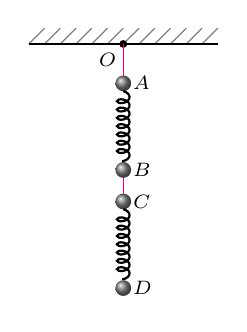
\begin{tikzpicture}[font=\scriptsize]
	\foreach \x in {-1.2,-1,...,1}
		\draw[gray] (\x,0)--++(.2,.2);
	\draw[thick] (-1.2,0)--(1.2,0);
	\fill (0,0) circle(.05);
	\draw[magenta] (0,0)--(0,-.6) (0,-1.5)--(0,-2.1);
	\shade[ball color=gray] (0,-.5)node[right]{\(A\)} circle(.1);
	\shade[ball color=gray] (0,-1.6)node[right]{\(B\)} circle(.1);
	\shade[ball color=gray] (0,-2)node[right]{\(C\)} circle(.1);
	\shade[ball color=gray] (0,-3.1)node[right]{\(D\)} circle(.1);
	\draw[thick,decoration={aspect=.6,segment length=3,amplitude=.8mm,coil},decorate] (0,-.6)--(0,-1.5);
	\draw[thick,decoration={aspect=.6,segment length=3,amplitude=.8mm,coil},decorate] (0,-2.1)--(0,-3);
	\node at(-.2,-.2){\(O\)};
\end{tikzpicture}
\begin{choices}
	\item \(g,1.5g\)
	\item \(2g,1.5g\)
	\item \(2g,0.5g\)
	\item \(g,0.5g\)
\end{choices}
\begin{answer}
	A\qquad 提示：
\end{answer}